% Options for packages loaded elsewhere
\PassOptionsToPackage{unicode}{hyperref}
\PassOptionsToPackage{hyphens}{url}
%
\documentclass[
]{article}
\usepackage{amsmath,amssymb}
\usepackage{iftex}
\ifPDFTeX
  \usepackage[T1]{fontenc}
  \usepackage[utf8]{inputenc}
  \usepackage{textcomp} % provide euro and other symbols
\else % if luatex or xetex
  \usepackage{unicode-math} % this also loads fontspec
  \defaultfontfeatures{Scale=MatchLowercase}
  \defaultfontfeatures[\rmfamily]{Ligatures=TeX,Scale=1}
\fi
\usepackage{lmodern}
\ifPDFTeX\else
  % xetex/luatex font selection
\fi
% Use upquote if available, for straight quotes in verbatim environments
\IfFileExists{upquote.sty}{\usepackage{upquote}}{}
\IfFileExists{microtype.sty}{% use microtype if available
  \usepackage[]{microtype}
  \UseMicrotypeSet[protrusion]{basicmath} % disable protrusion for tt fonts
}{}
\makeatletter
\@ifundefined{KOMAClassName}{% if non-KOMA class
  \IfFileExists{parskip.sty}{%
    \usepackage{parskip}
  }{% else
    \setlength{\parindent}{0pt}
    \setlength{\parskip}{6pt plus 2pt minus 1pt}}
}{% if KOMA class
  \KOMAoptions{parskip=half}}
\makeatother
\usepackage{xcolor}
\usepackage[margin=1in]{geometry}
\usepackage{color}
\usepackage{fancyvrb}
\newcommand{\VerbBar}{|}
\newcommand{\VERB}{\Verb[commandchars=\\\{\}]}
\DefineVerbatimEnvironment{Highlighting}{Verbatim}{commandchars=\\\{\}}
% Add ',fontsize=\small' for more characters per line
\usepackage{framed}
\definecolor{shadecolor}{RGB}{248,248,248}
\newenvironment{Shaded}{\begin{snugshade}}{\end{snugshade}}
\newcommand{\AlertTok}[1]{\textcolor[rgb]{0.94,0.16,0.16}{#1}}
\newcommand{\AnnotationTok}[1]{\textcolor[rgb]{0.56,0.35,0.01}{\textbf{\textit{#1}}}}
\newcommand{\AttributeTok}[1]{\textcolor[rgb]{0.13,0.29,0.53}{#1}}
\newcommand{\BaseNTok}[1]{\textcolor[rgb]{0.00,0.00,0.81}{#1}}
\newcommand{\BuiltInTok}[1]{#1}
\newcommand{\CharTok}[1]{\textcolor[rgb]{0.31,0.60,0.02}{#1}}
\newcommand{\CommentTok}[1]{\textcolor[rgb]{0.56,0.35,0.01}{\textit{#1}}}
\newcommand{\CommentVarTok}[1]{\textcolor[rgb]{0.56,0.35,0.01}{\textbf{\textit{#1}}}}
\newcommand{\ConstantTok}[1]{\textcolor[rgb]{0.56,0.35,0.01}{#1}}
\newcommand{\ControlFlowTok}[1]{\textcolor[rgb]{0.13,0.29,0.53}{\textbf{#1}}}
\newcommand{\DataTypeTok}[1]{\textcolor[rgb]{0.13,0.29,0.53}{#1}}
\newcommand{\DecValTok}[1]{\textcolor[rgb]{0.00,0.00,0.81}{#1}}
\newcommand{\DocumentationTok}[1]{\textcolor[rgb]{0.56,0.35,0.01}{\textbf{\textit{#1}}}}
\newcommand{\ErrorTok}[1]{\textcolor[rgb]{0.64,0.00,0.00}{\textbf{#1}}}
\newcommand{\ExtensionTok}[1]{#1}
\newcommand{\FloatTok}[1]{\textcolor[rgb]{0.00,0.00,0.81}{#1}}
\newcommand{\FunctionTok}[1]{\textcolor[rgb]{0.13,0.29,0.53}{\textbf{#1}}}
\newcommand{\ImportTok}[1]{#1}
\newcommand{\InformationTok}[1]{\textcolor[rgb]{0.56,0.35,0.01}{\textbf{\textit{#1}}}}
\newcommand{\KeywordTok}[1]{\textcolor[rgb]{0.13,0.29,0.53}{\textbf{#1}}}
\newcommand{\NormalTok}[1]{#1}
\newcommand{\OperatorTok}[1]{\textcolor[rgb]{0.81,0.36,0.00}{\textbf{#1}}}
\newcommand{\OtherTok}[1]{\textcolor[rgb]{0.56,0.35,0.01}{#1}}
\newcommand{\PreprocessorTok}[1]{\textcolor[rgb]{0.56,0.35,0.01}{\textit{#1}}}
\newcommand{\RegionMarkerTok}[1]{#1}
\newcommand{\SpecialCharTok}[1]{\textcolor[rgb]{0.81,0.36,0.00}{\textbf{#1}}}
\newcommand{\SpecialStringTok}[1]{\textcolor[rgb]{0.31,0.60,0.02}{#1}}
\newcommand{\StringTok}[1]{\textcolor[rgb]{0.31,0.60,0.02}{#1}}
\newcommand{\VariableTok}[1]{\textcolor[rgb]{0.00,0.00,0.00}{#1}}
\newcommand{\VerbatimStringTok}[1]{\textcolor[rgb]{0.31,0.60,0.02}{#1}}
\newcommand{\WarningTok}[1]{\textcolor[rgb]{0.56,0.35,0.01}{\textbf{\textit{#1}}}}
\usepackage{graphicx}
\makeatletter
\def\maxwidth{\ifdim\Gin@nat@width>\linewidth\linewidth\else\Gin@nat@width\fi}
\def\maxheight{\ifdim\Gin@nat@height>\textheight\textheight\else\Gin@nat@height\fi}
\makeatother
% Scale images if necessary, so that they will not overflow the page
% margins by default, and it is still possible to overwrite the defaults
% using explicit options in \includegraphics[width, height, ...]{}
\setkeys{Gin}{width=\maxwidth,height=\maxheight,keepaspectratio}
% Set default figure placement to htbp
\makeatletter
\def\fps@figure{htbp}
\makeatother
\setlength{\emergencystretch}{3em} % prevent overfull lines
\providecommand{\tightlist}{%
  \setlength{\itemsep}{0pt}\setlength{\parskip}{0pt}}
\setcounter{secnumdepth}{-\maxdimen} % remove section numbering
\ifLuaTeX
  \usepackage{selnolig}  % disable illegal ligatures
\fi
\usepackage{bookmark}
\IfFileExists{xurl.sty}{\usepackage{xurl}}{} % add URL line breaks if available
\urlstyle{same}
\hypersetup{
  pdftitle={Rangewide Analysis},
  pdfauthor={Andres N. Rosales},
  hidelinks,
  pdfcreator={LaTeX via pandoc}}

\title{Rangewide Analysis}
\author{Andres N. Rosales}
\date{2025-01-24}

\begin{document}
\maketitle

{
\setcounter{tocdepth}{2}
\tableofcontents
}
\section{Candidate Models}\label{candidate-models}

\textbf{Prediction 1}

Breeding regions declining in trend will be correlated with low
landscape heterogeneity and simplified agricultural landscapes.

\(Trend = Δ SHDI + Δ Edge Density + Δ Cropland + (1 | Location)\)

\textbf{Prediction 2}

Greater landscape heterogeneity will lower the negative effects of
landscape simplification on breeding trends. ``Is the effect of
landscape diversity on Upland Sandpiper population dynamics dependent on
the degree of simplification?''

\(Trend = Δ SHDI + Δ Cropland + Δ SHDI * Δ Cropland + (1 | Location)\)

\textbf{Prediction 3}

Forage agriculture and grasslands are associated with positive trends
and high abundance. ``How are trends in forage agriculture and
grasslands associated with trends and abundance of Upland Sandpiper?''

\(Trend = Δ Forage Ag + Δ Grassland + (1 | Location)\)

``Does configuration of forage and grassland habitats influence their
association with trends and abundance

\(Trend = Δ Forage Agriculture * Δ Forage Ag LPI + Δ Grassland *  Δ Grassland LPI + (1 | Location)\)

\textbf{Prediction 4}

Trends decline or become more variable with increasing distance from the
core breeding range. Conversely, trends will be more stable near the
core breeding region.

\(Trend = Periphery + (1 | Location)\)

\textbf{Prediction 5}

Geographical variation in abundance is driven by marginal habitat at the
periphery.

\(Trend = Periphery + Δ SHDI +  Δ Cropland + (1 | Location) + (1| Year)\)

\section{Response Distribution}\label{response-distribution}

Distribution of trend response variable.

\begin{Shaded}
\begin{Highlighting}[]
\FunctionTok{ggplot}\NormalTok{(upsabuff, }\FunctionTok{aes}\NormalTok{(}\AttributeTok{x =}\NormalTok{ abd\_trend)) }\SpecialCharTok{+}
  \FunctionTok{geom\_histogram}\NormalTok{(}\AttributeTok{bins =} \DecValTok{30}\NormalTok{, }\AttributeTok{fill =} \StringTok{"blue"}\NormalTok{, }\AttributeTok{color =} \StringTok{"black"}\NormalTok{) }\SpecialCharTok{+}
  \FunctionTok{theme\_minimal}\NormalTok{()}
\end{Highlighting}
\end{Shaded}

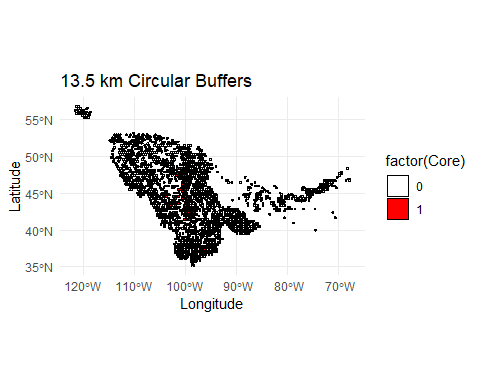
\includegraphics{NA_Analysis_files/figure-latex/unnamed-chunk-6-1.pdf}
Almost follows a normal distribution, but without trends that are zero
(stable) we observe biomodal. I could possibly look into adding a
categorical variable indicating increase or decrease. I need to explore
this more\ldots{}

\begin{Shaded}
\begin{Highlighting}[]
\CommentTok{\#add categorical variable to each location indicating increase or decrease}
\NormalTok{upsa\_trd}\SpecialCharTok{$}\NormalTok{trend\_dir }\OtherTok{\textless{}{-}} \FunctionTok{ifelse}\NormalTok{(upsa\_trd}\SpecialCharTok{$}\NormalTok{abd\_trend }\SpecialCharTok{\textgreater{}}\DecValTok{0}\NormalTok{, }\StringTok{"Increase"}\NormalTok{, }\StringTok{"Decrease"}\NormalTok{)}
\end{Highlighting}
\end{Shaded}

\begin{Shaded}
\begin{Highlighting}[]
\CommentTok{\#Distribution of abundance response variable. }
\FunctionTok{ggplot}\NormalTok{(upsabuff, }\FunctionTok{aes}\NormalTok{(}\AttributeTok{x =}\NormalTok{ abd)) }\SpecialCharTok{+}
  \FunctionTok{geom\_histogram}\NormalTok{(}\AttributeTok{bins =} \DecValTok{30}\NormalTok{, }\AttributeTok{fill =} \StringTok{"blue"}\NormalTok{, }\AttributeTok{color =} \StringTok{"black"}\NormalTok{) }\SpecialCharTok{+}
  \FunctionTok{theme\_minimal}\NormalTok{()}
\end{Highlighting}
\end{Shaded}

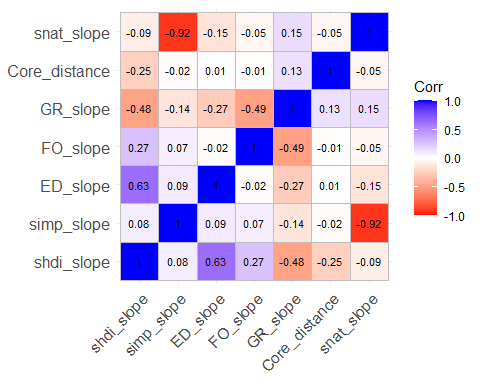
\includegraphics{NA_Analysis_files/figure-latex/unnamed-chunk-8-1.pdf}
Distribution of abundance estimates.

\section{Predictor relationships}\label{predictor-relationships}

Correlation matric before aggregating predictors.

\begin{Shaded}
\begin{Highlighting}[]
\FunctionTok{library}\NormalTok{(ggcorrplot)}
\end{Highlighting}
\end{Shaded}

\begin{verbatim}
## Warning: package 'ggcorrplot' was built under R version 4.4.2
\end{verbatim}

\begin{Shaded}
\begin{Highlighting}[]
\CommentTok{\# List of predictors to include}
\NormalTok{predictors }\OtherTok{\textless{}{-}} \FunctionTok{c}\NormalTok{(}
   \StringTok{"lpi\_c11\_Grassland"}\NormalTok{, }\StringTok{"shdi\_cNA\_NA"}\NormalTok{, }\StringTok{"lpi\_c09\_Forage"}\NormalTok{, }\StringTok{"pland\_c02\_Ag"}\NormalTok{, }\StringTok{"ed\_cNA\_NA"}
\NormalTok{)}

\CommentTok{\# Filter dataset}
\NormalTok{filtered\_data }\OtherTok{\textless{}{-}}\NormalTok{ all\_lsm }\SpecialCharTok{\%\textgreater{}\%}
\NormalTok{  dplyr}\SpecialCharTok{::}\FunctionTok{select}\NormalTok{(}\FunctionTok{all\_of}\NormalTok{(predictors))}

\CommentTok{\# Compute correlation matrix}
\NormalTok{cor\_matrix }\OtherTok{\textless{}{-}} \FunctionTok{cor}\NormalTok{(filtered\_data, }\AttributeTok{use =} \StringTok{"complete.obs"}\NormalTok{, }\AttributeTok{method =} \StringTok{"pearson"}\NormalTok{)}

\CommentTok{\# Visualize the correlation matrix}
\FunctionTok{ggcorrplot}\NormalTok{(cor\_matrix, }\AttributeTok{lab =} \ConstantTok{TRUE}\NormalTok{, }\AttributeTok{lab\_size =} \DecValTok{3}\NormalTok{, }\AttributeTok{colors =} \FunctionTok{c}\NormalTok{(}\StringTok{"red"}\NormalTok{, }\StringTok{"white"}\NormalTok{, }\StringTok{"blue"}\NormalTok{))}
\end{Highlighting}
\end{Shaded}

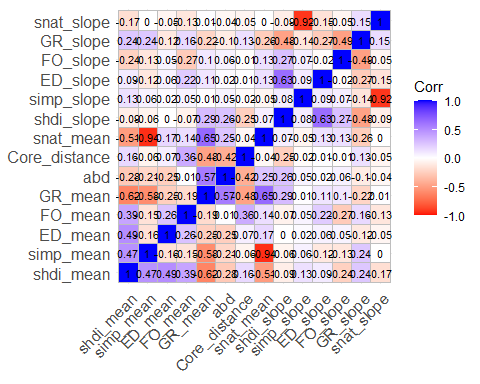
\includegraphics{NA_Analysis_files/figure-latex/unnamed-chunk-9-1.pdf}

I still need to determine a pearsons correlation coefficient threshold
to report. Some literature has used 0.7 and I will go with that for now.
I still need to develop a better backing for this and if this is
something I will continue to use going forward\ldots{}

\subsection{Shannon Diversity Index}\label{shannon-diversity-index}

I want to use the slope of a linear regression for SHDI
\textasciitilde{} year for every location as a proxy for change in SHDI.
I will need to confirm SHDI changes in linearly. fit lm and gam and
compare fit for slope of SHDI as explanatory predictor

\begin{Shaded}
\begin{Highlighting}[]
\NormalTok{shdi\_lmm }\OtherTok{\textless{}{-}} \FunctionTok{lmer}\NormalTok{(shdi\_cNA\_NA }\SpecialCharTok{\textasciitilde{}}\NormalTok{ year }\SpecialCharTok{+}\NormalTok{ (}\DecValTok{1}\SpecialCharTok{|}\NormalTok{srd\_id), }\AttributeTok{data =}\NormalTok{ all\_lsm)}
\FunctionTok{summary}\NormalTok{(shdi\_lmm)}
\end{Highlighting}
\end{Shaded}

\begin{verbatim}
## Linear mixed model fit by REML ['lmerMod']
## Formula: shdi_cNA_NA ~ year + (1 | srd_id)
##    Data: all_lsm
## 
## REML criterion at convergence: -34837.1
## 
## Scaled residuals: 
##      Min       1Q   Median       3Q      Max 
## -14.0486  -0.4342  -0.0162   0.4080  10.1691 
## 
## Random effects:
##  Groups   Name        Variance Std.Dev.
##  srd_id   (Intercept) 0.149392 0.38651 
##  Residual             0.007152 0.08457 
## Number of obs: 21681, groups:  srd_id, 1971
## 
## Fixed effects:
##               Estimate Std. Error t value
## (Intercept) -8.9275736  0.3664480  -24.36
## year         0.0051451  0.0001816   28.33
## 
## Correlation of Fixed Effects:
##      (Intr)
## year -1.000
\end{verbatim}

\begin{Shaded}
\begin{Highlighting}[]
\NormalTok{shdi\_gamm }\OtherTok{\textless{}{-}} \FunctionTok{gam}\NormalTok{(shdi\_cNA\_NA }\SpecialCharTok{\textasciitilde{}} \FunctionTok{s}\NormalTok{(year, }\AttributeTok{k=}\DecValTok{10}\NormalTok{) }\SpecialCharTok{+}\NormalTok{ srd\_id, }\AttributeTok{method=}\StringTok{"REML"}\NormalTok{, }\AttributeTok{data =}\NormalTok{ all\_lsm)}
\FunctionTok{summary}\NormalTok{(shdi\_gamm)}
\end{Highlighting}
\end{Shaded}

\begin{verbatim}
## 
## Family: gaussian 
## Link function: identity 
## 
## Formula:
## shdi_cNA_NA ~ s(year, k = 10) + srd_id
## 
## Parametric coefficients:
##               Estimate Std. Error t value Pr(>|t|)    
## (Intercept)  2.443e+00  2.672e-02   91.42   <2e-16 ***
## srd_id      -3.503e-06  9.382e-08  -37.33   <2e-16 ***
## ---
## Signif. codes:  0 '***' 0.001 '**' 0.01 '*' 0.05 '.' 0.1 ' ' 1
## 
## Approximate significance of smooth terms:
##           edf Ref.df     F p-value    
## s(year) 4.291  5.282 12.09  <2e-16 ***
## ---
## Signif. codes:  0 '***' 0.001 '**' 0.01 '*' 0.05 '.' 0.1 ' ' 1
## 
## R-sq.(adj) =  0.063   Deviance explained = 6.32%
## -REML = 9997.3  Scale est. = 0.14687   n = 21681
\end{verbatim}

\begin{Shaded}
\begin{Highlighting}[]
\FunctionTok{AIC}\NormalTok{(shdi\_lmm, shdi\_gamm)}
\end{Highlighting}
\end{Shaded}

\begin{verbatim}
##                 df       AIC
## shdi_lmm  4.000000 -34829.10
## shdi_gamm 8.281729  19949.43
\end{verbatim}

Big difference in AIC values when comparing GAM and lm model. the
relationships of each location likely follow a linear relationship over
years, allowing it to be representative of the change in diversity over
time.

Calculate change in SHDI using linear regression. THis will be used as a
predictor representing the change in diversity over the trend period

\begin{Shaded}
\begin{Highlighting}[]
\CommentTok{\#Slope and intercept}
\NormalTok{shdi\_slopes }\OtherTok{\textless{}{-}}\NormalTok{ all\_lsm }\SpecialCharTok{\%\textgreater{}\%}
  \FunctionTok{group\_by}\NormalTok{(srd\_id) }\SpecialCharTok{\%\textgreater{}\%}
  \FunctionTok{summarize}\NormalTok{(}
    \AttributeTok{shdi\_slope =} \FunctionTok{coef}\NormalTok{(}\FunctionTok{lm}\NormalTok{(shdi\_cNA\_NA }\SpecialCharTok{\textasciitilde{}}\NormalTok{ year))[}\DecValTok{2}\NormalTok{],  }
    \AttributeTok{shdi\_intercept =} \FunctionTok{coef}\NormalTok{(}\FunctionTok{lm}\NormalTok{(shdi\_cNA\_NA }\SpecialCharTok{\textasciitilde{}}\NormalTok{ year))[}\DecValTok{1}\NormalTok{] }
\NormalTok{  )}

\NormalTok{upsa\_trd }\OtherTok{\textless{}{-}}\NormalTok{ shdi\_slopes }\SpecialCharTok{\%\textgreater{}\%}
  \FunctionTok{left\_join}\NormalTok{(upsa\_trd, }\AttributeTok{by =} \FunctionTok{c}\NormalTok{(}\StringTok{"srd\_id"}\NormalTok{))}
\end{Highlighting}
\end{Shaded}

add mean and standard deviation of shdi for each location

\begin{Shaded}
\begin{Highlighting}[]
\CommentTok{\#Mean}
\NormalTok{mean\_shdi }\OtherTok{\textless{}{-}}\NormalTok{ all\_lsm }\SpecialCharTok{\%\textgreater{}\%}
  \FunctionTok{group\_by}\NormalTok{(srd\_id) }\SpecialCharTok{\%\textgreater{}\%}
  \FunctionTok{summarize}\NormalTok{(}\AttributeTok{mean\_shdi =} \FunctionTok{mean}\NormalTok{(shdi\_cNA\_NA, }\AttributeTok{na.rm =} \ConstantTok{TRUE}\NormalTok{))}
\NormalTok{upsa\_trd }\OtherTok{\textless{}{-}}\NormalTok{ mean\_shdi }\SpecialCharTok{\%\textgreater{}\%}
  \FunctionTok{left\_join}\NormalTok{(upsa\_trd, }\AttributeTok{by =} \StringTok{"srd\_id"}\NormalTok{)}
\CommentTok{\#Standard Dev}
\NormalTok{sd\_shdi }\OtherTok{\textless{}{-}}\NormalTok{ all\_lsm }\SpecialCharTok{\%\textgreater{}\%}
  \FunctionTok{group\_by}\NormalTok{(srd\_id) }\SpecialCharTok{\%\textgreater{}\%}
  \FunctionTok{summarize}\NormalTok{(}\AttributeTok{sd\_shdi =} \FunctionTok{sd}\NormalTok{(shdi\_cNA\_NA, }\AttributeTok{na.rm =} \ConstantTok{TRUE}\NormalTok{))}

\NormalTok{upsa\_trd }\OtherTok{\textless{}{-}}\NormalTok{ sd\_shdi }\SpecialCharTok{\%\textgreater{}\%}
  \FunctionTok{left\_join}\NormalTok{(upsa\_trd, }\AttributeTok{by =} \StringTok{"srd\_id"}\NormalTok{)}
\end{Highlighting}
\end{Shaded}

\begin{Shaded}
\begin{Highlighting}[]
\FunctionTok{ggplot}\NormalTok{(upsa\_trd, }\FunctionTok{aes}\NormalTok{(}\AttributeTok{x =}\NormalTok{ shdi\_slope, }\AttributeTok{y =}\NormalTok{ abd\_trend)) }\SpecialCharTok{+}
  \FunctionTok{geom\_point}\NormalTok{(}\AttributeTok{color =} \StringTok{"blue"}\NormalTok{, }\AttributeTok{alpha =} \FloatTok{0.3}\NormalTok{, }\AttributeTok{size =} \DecValTok{2}\NormalTok{) }\SpecialCharTok{+}  
  \FunctionTok{geom\_smooth}\NormalTok{(}\AttributeTok{method =} \StringTok{"lm"}\NormalTok{, }\AttributeTok{color =} \StringTok{"red"}\NormalTok{, }\AttributeTok{se =} \ConstantTok{TRUE}\NormalTok{, }\AttributeTok{linetype =} \StringTok{"dashed"}\NormalTok{) }\SpecialCharTok{+} 
  \FunctionTok{labs}\NormalTok{(}
    \AttributeTok{title =} \StringTok{"Relationship Between SHDI Slope and Trend"}\NormalTok{,}
    \AttributeTok{x =} \StringTok{"Slope of SHDI (Change over Time)"}\NormalTok{,}
    \AttributeTok{y =} \StringTok{"Trend"}
\NormalTok{  ) }\SpecialCharTok{+}
  \FunctionTok{theme\_minimal}\NormalTok{() }\SpecialCharTok{+}
  \FunctionTok{theme}\NormalTok{(}
    \AttributeTok{plot.title =} \FunctionTok{element\_text}\NormalTok{(}\AttributeTok{hjust =} \FloatTok{0.5}\NormalTok{, }\AttributeTok{size =} \DecValTok{16}\NormalTok{),}
    \AttributeTok{axis.title =} \FunctionTok{element\_text}\NormalTok{(}\AttributeTok{size =} \DecValTok{14}\NormalTok{),}
    \AttributeTok{axis.text =} \FunctionTok{element\_text}\NormalTok{(}\AttributeTok{size =} \DecValTok{12}\NormalTok{)}
\NormalTok{  )}
\end{Highlighting}
\end{Shaded}

\begin{verbatim}
## `geom_smooth()` using formula = 'y ~ x'
\end{verbatim}

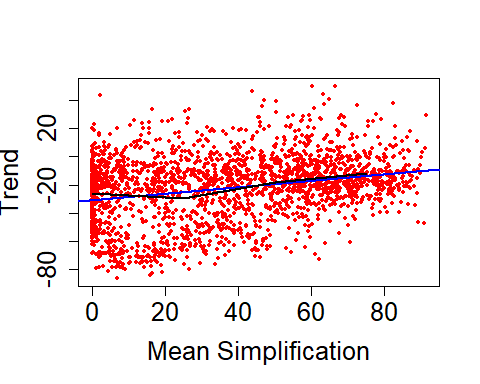
\includegraphics{NA_Analysis_files/figure-latex/unnamed-chunk-14-1.pdf}

Figure reveals mostly linear with some deviation along the edges. Test
lm and gam model to determine best fit.

\begin{Shaded}
\begin{Highlighting}[]
\NormalTok{shdilm\_model }\OtherTok{\textless{}{-}} \FunctionTok{lm}\NormalTok{(abd\_trend }\SpecialCharTok{\textasciitilde{}}\NormalTok{ shdi\_slope, }\AttributeTok{data =}\NormalTok{ upsa\_trd)}
\FunctionTok{plot}\NormalTok{(}\FunctionTok{fitted}\NormalTok{(shdilm\_model), }\FunctionTok{residuals}\NormalTok{(shdilm\_model), }\AttributeTok{main =} \StringTok{"Residuals vs Fitted"}\NormalTok{)}
\FunctionTok{abline}\NormalTok{(}\AttributeTok{h =} \DecValTok{0}\NormalTok{, }\AttributeTok{col =} \StringTok{"red"}\NormalTok{)}
\end{Highlighting}
\end{Shaded}

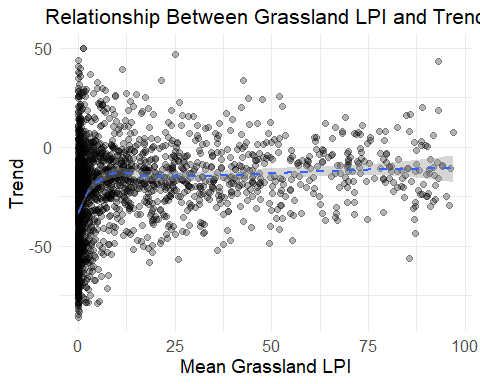
\includegraphics{NA_Analysis_files/figure-latex/unnamed-chunk-15-1.pdf}

\begin{Shaded}
\begin{Highlighting}[]
\NormalTok{shdigam\_model }\OtherTok{\textless{}{-}} \FunctionTok{gam}\NormalTok{(abd\_trend }\SpecialCharTok{\textasciitilde{}} \FunctionTok{s}\NormalTok{(shdi\_slope), }\AttributeTok{data =}\NormalTok{ upsa\_trd)}
\FunctionTok{summary}\NormalTok{(shdilm\_model)}
\end{Highlighting}
\end{Shaded}

\begin{verbatim}
## 
## Call:
## lm(formula = abd_trend ~ shdi_slope, data = upsa_trd)
## 
## Residuals:
##     Min      1Q  Median      3Q     Max 
## -61.388 -20.679  -3.738   7.770 172.118 
## 
## Coefficients:
##             Estimate Std. Error t value Pr(>|t|)    
## (Intercept) -23.7973     0.7742 -30.738  < 2e-16 ***
## shdi_slope  308.4663    44.9874   6.857  9.4e-12 ***
## ---
## Signif. codes:  0 '***' 0.001 '**' 0.01 '*' 0.05 '.' 0.1 ' ' 1
## 
## Residual standard error: 32.8 on 1969 degrees of freedom
## Multiple R-squared:  0.02332,    Adjusted R-squared:  0.02282 
## F-statistic: 47.01 on 1 and 1969 DF,  p-value: 9.396e-12
\end{verbatim}

\begin{Shaded}
\begin{Highlighting}[]
\FunctionTok{summary}\NormalTok{(shdigam\_model)}
\end{Highlighting}
\end{Shaded}

\begin{verbatim}
## 
## Family: gaussian 
## Link function: identity 
## 
## Formula:
## abd_trend ~ s(shdi_slope)
## 
## Parametric coefficients:
##             Estimate Std. Error t value Pr(>|t|)    
## (Intercept) -22.2102     0.7379   -30.1   <2e-16 ***
## ---
## Signif. codes:  0 '***' 0.001 '**' 0.01 '*' 0.05 '.' 0.1 ' ' 1
## 
## Approximate significance of smooth terms:
##                 edf Ref.df     F p-value    
## s(shdi_slope) 2.633  3.388 15.13  <2e-16 ***
## ---
## Signif. codes:  0 '***' 0.001 '**' 0.01 '*' 0.05 '.' 0.1 ' ' 1
## 
## R-sq.(adj) =  0.0252   Deviance explained = 2.65%
## GCV = 1075.1  Scale est. = 1073.1    n = 1971
\end{verbatim}

\begin{Shaded}
\begin{Highlighting}[]
\CommentTok{\# Compare lm and gam}
\FunctionTok{AIC}\NormalTok{(shdilm\_model, shdigam\_model)}
\end{Highlighting}
\end{Shaded}

\begin{verbatim}
##                    df      AIC
## shdilm_model  3.00000 19356.62
## shdigam_model 4.63294 19353.40
\end{verbatim}

Slight improvement of fit with the GAM model. However, since it is small
it might be ok to assume linear relationship.

\subsection{Landscape Simplification}\label{landscape-simplification}

calculate slope of landscape simplification over 11 years

\begin{Shaded}
\begin{Highlighting}[]
\NormalTok{simp\_slopes }\OtherTok{\textless{}{-}}\NormalTok{ all\_lsm }\SpecialCharTok{\%\textgreater{}\%}
  \FunctionTok{group\_by}\NormalTok{(srd\_id) }\SpecialCharTok{\%\textgreater{}\%}
  \FunctionTok{summarize}\NormalTok{(}
    \AttributeTok{simp\_slope =} \FunctionTok{coef}\NormalTok{(}\FunctionTok{lm}\NormalTok{(pland\_c02\_Ag }\SpecialCharTok{\textasciitilde{}}\NormalTok{ year))[}\DecValTok{2}\NormalTok{],  }
    \AttributeTok{simp\_intercept =} \FunctionTok{coef}\NormalTok{(}\FunctionTok{lm}\NormalTok{(pland\_c02\_Ag }\SpecialCharTok{\textasciitilde{}}\NormalTok{ year))[}\DecValTok{1}\NormalTok{] }
\NormalTok{  )}

\NormalTok{upsa\_trd }\OtherTok{\textless{}{-}}\NormalTok{ simp\_slopes }\SpecialCharTok{\%\textgreater{}\%}
  \FunctionTok{left\_join}\NormalTok{(upsa\_trd, }\AttributeTok{by =} \FunctionTok{c}\NormalTok{(}\StringTok{"srd\_id"}\NormalTok{))}
\end{Highlighting}
\end{Shaded}

plot simplification slope against trend

\begin{Shaded}
\begin{Highlighting}[]
\FunctionTok{ggplot}\NormalTok{(upsa\_trd, }\FunctionTok{aes}\NormalTok{(}\AttributeTok{x =}\NormalTok{ simp\_slope, }\AttributeTok{y =}\NormalTok{ abd\_trend)) }\SpecialCharTok{+}
  \FunctionTok{geom\_point}\NormalTok{(}\AttributeTok{color =} \StringTok{"blue"}\NormalTok{, }\AttributeTok{alpha =} \FloatTok{0.3}\NormalTok{, }\AttributeTok{size =} \DecValTok{2}\NormalTok{) }\SpecialCharTok{+}  
  \FunctionTok{geom\_smooth}\NormalTok{(}\AttributeTok{method =} \StringTok{"gam"}\NormalTok{, }\AttributeTok{color =} \StringTok{"red"}\NormalTok{, }\AttributeTok{se =} \ConstantTok{TRUE}\NormalTok{, }\AttributeTok{linetype =} \StringTok{"dashed"}\NormalTok{) }\SpecialCharTok{+} 
  \FunctionTok{labs}\NormalTok{(}
    \AttributeTok{title =} \StringTok{"Relationship Between SHDI Slope and Trend"}\NormalTok{,}
    \AttributeTok{x =} \StringTok{"Slope of SHDI (Change over Time)"}\NormalTok{,}
    \AttributeTok{y =} \StringTok{"Trend"}
\NormalTok{  ) }\SpecialCharTok{+}
  \FunctionTok{theme\_minimal}\NormalTok{() }\SpecialCharTok{+}
  \FunctionTok{theme}\NormalTok{(}
    \AttributeTok{plot.title =} \FunctionTok{element\_text}\NormalTok{(}\AttributeTok{hjust =} \FloatTok{0.5}\NormalTok{, }\AttributeTok{size =} \DecValTok{16}\NormalTok{),}
    \AttributeTok{axis.title =} \FunctionTok{element\_text}\NormalTok{(}\AttributeTok{size =} \DecValTok{14}\NormalTok{),}
    \AttributeTok{axis.text =} \FunctionTok{element\_text}\NormalTok{(}\AttributeTok{size =} \DecValTok{12}\NormalTok{)}
\NormalTok{  )}
\end{Highlighting}
\end{Shaded}

\begin{verbatim}
## `geom_smooth()` using formula = 'y ~ s(x, bs = "cs")'
\end{verbatim}

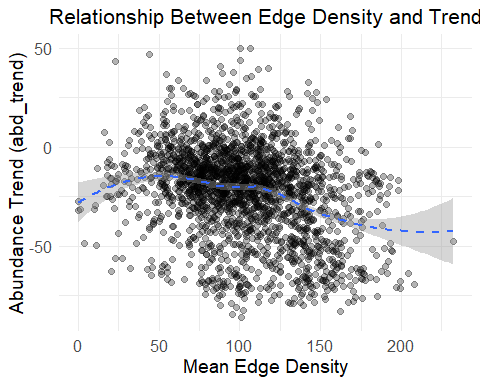
\includegraphics{NA_Analysis_files/figure-latex/unnamed-chunk-17-1.pdf}

\begin{Shaded}
\begin{Highlighting}[]
\NormalTok{simplm\_model }\OtherTok{\textless{}{-}} \FunctionTok{lm}\NormalTok{(abd\_trend }\SpecialCharTok{\textasciitilde{}}\NormalTok{ simp\_slope, }\AttributeTok{data =}\NormalTok{ upsa\_trd)}
\FunctionTok{plot}\NormalTok{(}\FunctionTok{fitted}\NormalTok{(simplm\_model), }\FunctionTok{residuals}\NormalTok{(simplm\_model), }\AttributeTok{main =} \StringTok{"Residuals vs Fitted"}\NormalTok{)}
\FunctionTok{abline}\NormalTok{(}\AttributeTok{h =} \DecValTok{0}\NormalTok{, }\AttributeTok{col =} \StringTok{"red"}\NormalTok{)}
\end{Highlighting}
\end{Shaded}

\includegraphics{NA_Analysis_files/figure-latex/unnamed-chunk-18-1.pdf}

\begin{Shaded}
\begin{Highlighting}[]
\NormalTok{simpgam\_model }\OtherTok{\textless{}{-}} \FunctionTok{gam}\NormalTok{(abd\_trend }\SpecialCharTok{\textasciitilde{}} \FunctionTok{s}\NormalTok{(simp\_slope), }\AttributeTok{data =}\NormalTok{ upsa\_trd)}
\FunctionTok{summary}\NormalTok{(simplm\_model)}
\end{Highlighting}
\end{Shaded}

\begin{verbatim}
## 
## Call:
## lm(formula = abd_trend ~ simp_slope, data = upsa_trd)
## 
## Residuals:
##     Min      1Q  Median      3Q     Max 
## -62.918 -21.016  -2.607   8.113 160.319 
## 
## Coefficients:
##             Estimate Std. Error t value Pr(>|t|)    
## (Intercept) -23.4372     0.8155 -28.740  < 2e-16 ***
## simp_slope    5.4440     1.4719   3.699 0.000223 ***
## ---
## Signif. codes:  0 '***' 0.001 '**' 0.01 '*' 0.05 '.' 0.1 ' ' 1
## 
## Residual standard error: 33.07 on 1969 degrees of freedom
## Multiple R-squared:  0.0069, Adjusted R-squared:  0.006395 
## F-statistic: 13.68 on 1 and 1969 DF,  p-value: 0.0002227
\end{verbatim}

\begin{Shaded}
\begin{Highlighting}[]
\FunctionTok{summary}\NormalTok{(simpgam\_model)}
\end{Highlighting}
\end{Shaded}

\begin{verbatim}
## 
## Family: gaussian 
## Link function: identity 
## 
## Formula:
## abd_trend ~ s(simp_slope)
## 
## Parametric coefficients:
##             Estimate Std. Error t value Pr(>|t|)    
## (Intercept) -22.2102     0.7428   -29.9   <2e-16 ***
## ---
## Signif. codes:  0 '***' 0.001 '**' 0.01 '*' 0.05 '.' 0.1 ' ' 1
## 
## Approximate significance of smooth terms:
##                 edf Ref.df     F  p-value    
## s(simp_slope) 2.977  3.812 6.359 7.28e-05 ***
## ---
## Signif. codes:  0 '***' 0.001 '**' 0.01 '*' 0.05 '.' 0.1 ' ' 1
## 
## R-sq.(adj) =  0.0122   Deviance explained = 1.37%
## GCV = 1089.7  Scale est. = 1087.5    n = 1971
\end{verbatim}

\begin{Shaded}
\begin{Highlighting}[]
\CommentTok{\# Compare lm and gam}
\FunctionTok{AIC}\NormalTok{(simplm\_model, simpgam\_model)}
\end{Highlighting}
\end{Shaded}

\begin{verbatim}
##                    df      AIC
## simplm_model  3.00000 19389.49
## simpgam_model 4.97683 19379.94
\end{verbatim}

\subsection{LPI Grassland}\label{lpi-grassland}

calculate the slope and average LPI for each location

\begin{Shaded}
\begin{Highlighting}[]
\CommentTok{\#Slope}
\NormalTok{GLPI\_slopes }\OtherTok{\textless{}{-}}\NormalTok{ all\_lsm }\SpecialCharTok{\%\textgreater{}\%}
  \FunctionTok{group\_by}\NormalTok{(srd\_id) }\SpecialCharTok{\%\textgreater{}\%}
  \FunctionTok{summarize}\NormalTok{(}
    \AttributeTok{GLPI\_slope =} \FunctionTok{coef}\NormalTok{(}\FunctionTok{lm}\NormalTok{(lpi\_c11\_Grassland }\SpecialCharTok{\textasciitilde{}}\NormalTok{ year))[}\DecValTok{2}\NormalTok{],  }
    \AttributeTok{GLPI\_intercept =} \FunctionTok{coef}\NormalTok{(}\FunctionTok{lm}\NormalTok{(lpi\_c11\_Grassland }\SpecialCharTok{\textasciitilde{}}\NormalTok{ year))[}\DecValTok{1}\NormalTok{] }
\NormalTok{  )}
\NormalTok{upsa\_trd }\OtherTok{\textless{}{-}}\NormalTok{ GLPI\_slopes }\SpecialCharTok{\%\textgreater{}\%}
  \FunctionTok{left\_join}\NormalTok{(upsa\_trd, }\AttributeTok{by =} \FunctionTok{c}\NormalTok{(}\StringTok{"srd\_id"}\NormalTok{))}

\CommentTok{\#Mean}
\NormalTok{mean\_GLPI }\OtherTok{\textless{}{-}}\NormalTok{ all\_lsm }\SpecialCharTok{\%\textgreater{}\%}
  \FunctionTok{group\_by}\NormalTok{(srd\_id) }\SpecialCharTok{\%\textgreater{}\%}
  \FunctionTok{summarize}\NormalTok{(}\AttributeTok{mean\_GLPI =} \FunctionTok{mean}\NormalTok{(lpi\_c11\_Grassland, }\AttributeTok{na.rm =} \ConstantTok{TRUE}\NormalTok{))}
\NormalTok{upsa\_trd }\OtherTok{\textless{}{-}}\NormalTok{ mean\_GLPI }\SpecialCharTok{\%\textgreater{}\%}
  \FunctionTok{left\_join}\NormalTok{(upsa\_trd, }\AttributeTok{by =} \StringTok{"srd\_id"}\NormalTok{)}
\end{Highlighting}
\end{Shaded}

Plot trend \textasciitilde{} slope and trend \textasciitilde{} Mean

\begin{Shaded}
\begin{Highlighting}[]
\FunctionTok{ggplot}\NormalTok{(upsa\_trd, }\FunctionTok{aes}\NormalTok{(}\AttributeTok{x =}\NormalTok{ GLPI\_slope, }\AttributeTok{y =}\NormalTok{ abd\_trend)) }\SpecialCharTok{+}
  \FunctionTok{geom\_point}\NormalTok{(}\AttributeTok{color =} \StringTok{"blue"}\NormalTok{, }\AttributeTok{alpha =} \FloatTok{0.3}\NormalTok{, }\AttributeTok{size =} \DecValTok{2}\NormalTok{) }\SpecialCharTok{+}  
  \FunctionTok{geom\_smooth}\NormalTok{(}\AttributeTok{method =} \StringTok{"lm"}\NormalTok{, }\AttributeTok{color =} \StringTok{"red"}\NormalTok{, }\AttributeTok{se =} \ConstantTok{TRUE}\NormalTok{, }\AttributeTok{linetype =} \StringTok{"dashed"}\NormalTok{) }\SpecialCharTok{+} 
  \FunctionTok{labs}\NormalTok{(}
    \AttributeTok{title =} \StringTok{"Relationship Between Grassland LPI and Trend"}\NormalTok{,}
    \AttributeTok{x =} \StringTok{"Slope of Grassland LPI (Change over Time)"}\NormalTok{,}
    \AttributeTok{y =} \StringTok{"Trend"}
\NormalTok{  ) }\SpecialCharTok{+}
  \FunctionTok{theme\_minimal}\NormalTok{() }\SpecialCharTok{+}
  \FunctionTok{theme}\NormalTok{(}
    \AttributeTok{plot.title =} \FunctionTok{element\_text}\NormalTok{(}\AttributeTok{hjust =} \FloatTok{0.5}\NormalTok{, }\AttributeTok{size =} \DecValTok{16}\NormalTok{),}
    \AttributeTok{axis.title =} \FunctionTok{element\_text}\NormalTok{(}\AttributeTok{size =} \DecValTok{14}\NormalTok{),}
    \AttributeTok{axis.text =} \FunctionTok{element\_text}\NormalTok{(}\AttributeTok{size =} \DecValTok{12}\NormalTok{)}
\NormalTok{  )}
\end{Highlighting}
\end{Shaded}

\begin{verbatim}
## `geom_smooth()` using formula = 'y ~ x'
\end{verbatim}

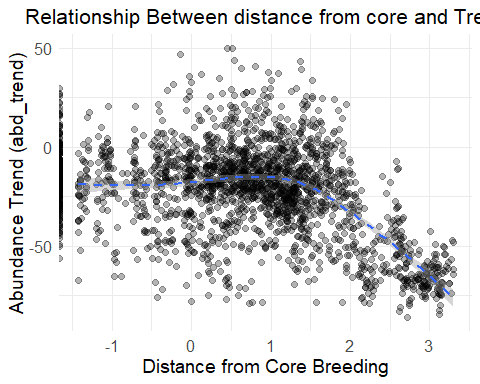
\includegraphics{NA_Analysis_files/figure-latex/unnamed-chunk-20-1.pdf}

\begin{Shaded}
\begin{Highlighting}[]
\FunctionTok{ggplot}\NormalTok{(upsa\_trd, }\FunctionTok{aes}\NormalTok{(}\AttributeTok{x =}\NormalTok{ mean\_GLPI, }\AttributeTok{y =}\NormalTok{ abd\_trend)) }\SpecialCharTok{+}
  \FunctionTok{geom\_point}\NormalTok{(}\AttributeTok{color =} \StringTok{"blue"}\NormalTok{, }\AttributeTok{alpha =} \FloatTok{0.3}\NormalTok{, }\AttributeTok{size =} \DecValTok{2}\NormalTok{) }\SpecialCharTok{+}  
  \FunctionTok{geom\_smooth}\NormalTok{(}\AttributeTok{method =} \StringTok{"lm"}\NormalTok{, }\AttributeTok{color =} \StringTok{"red"}\NormalTok{, }\AttributeTok{se =} \ConstantTok{TRUE}\NormalTok{, }\AttributeTok{linetype =} \StringTok{"dashed"}\NormalTok{) }\SpecialCharTok{+} 
  \FunctionTok{labs}\NormalTok{(}
    \AttributeTok{title =} \StringTok{"Relationship Between Grassland LPI and Trend"}\NormalTok{,}
    \AttributeTok{x =} \StringTok{"Slope of Grassland LPI (Change over Time)"}\NormalTok{,}
    \AttributeTok{y =} \StringTok{"Trend"}
\NormalTok{  ) }\SpecialCharTok{+}
  \FunctionTok{theme\_minimal}\NormalTok{() }\SpecialCharTok{+}
  \FunctionTok{theme}\NormalTok{(}
    \AttributeTok{plot.title =} \FunctionTok{element\_text}\NormalTok{(}\AttributeTok{hjust =} \FloatTok{0.5}\NormalTok{, }\AttributeTok{size =} \DecValTok{16}\NormalTok{),}
    \AttributeTok{axis.title =} \FunctionTok{element\_text}\NormalTok{(}\AttributeTok{size =} \DecValTok{14}\NormalTok{),}
    \AttributeTok{axis.text =} \FunctionTok{element\_text}\NormalTok{(}\AttributeTok{size =} \DecValTok{12}\NormalTok{)}
\NormalTok{  )}
\end{Highlighting}
\end{Shaded}

\begin{verbatim}
## `geom_smooth()` using formula = 'y ~ x'
\end{verbatim}

\includegraphics{NA_Analysis_files/figure-latex/unnamed-chunk-20-2.pdf}

\subsection{LPI Forage}\label{lpi-forage}

calculate the slope and average LPI for each location

\begin{Shaded}
\begin{Highlighting}[]
\CommentTok{\#Slope}
\NormalTok{FLPI\_slopes }\OtherTok{\textless{}{-}}\NormalTok{ all\_lsm }\SpecialCharTok{\%\textgreater{}\%}
  \FunctionTok{group\_by}\NormalTok{(srd\_id) }\SpecialCharTok{\%\textgreater{}\%}
  \FunctionTok{summarize}\NormalTok{(}
    \AttributeTok{FLPI\_slope =} \FunctionTok{coef}\NormalTok{(}\FunctionTok{lm}\NormalTok{(lpi\_c09\_Forage }\SpecialCharTok{\textasciitilde{}}\NormalTok{ year))[}\DecValTok{2}\NormalTok{],  }
    \AttributeTok{FLPI\_intercept =} \FunctionTok{coef}\NormalTok{(}\FunctionTok{lm}\NormalTok{(lpi\_c09\_Forage }\SpecialCharTok{\textasciitilde{}}\NormalTok{ year))[}\DecValTok{1}\NormalTok{] }
\NormalTok{  )}
\NormalTok{upsa\_trd }\OtherTok{\textless{}{-}}\NormalTok{ FLPI\_slopes }\SpecialCharTok{\%\textgreater{}\%}
  \FunctionTok{left\_join}\NormalTok{(upsa\_trd, }\AttributeTok{by =} \FunctionTok{c}\NormalTok{(}\StringTok{"srd\_id"}\NormalTok{))}

\CommentTok{\#Mean}
\NormalTok{mean\_FLPI }\OtherTok{\textless{}{-}}\NormalTok{ all\_lsm }\SpecialCharTok{\%\textgreater{}\%}
  \FunctionTok{group\_by}\NormalTok{(srd\_id) }\SpecialCharTok{\%\textgreater{}\%}
  \FunctionTok{summarize}\NormalTok{(}\AttributeTok{mean\_FLPI =} \FunctionTok{mean}\NormalTok{(lpi\_c09\_Forage, }\AttributeTok{na.rm =} \ConstantTok{TRUE}\NormalTok{))}
\NormalTok{upsa\_trd }\OtherTok{\textless{}{-}}\NormalTok{ mean\_FLPI }\SpecialCharTok{\%\textgreater{}\%}
  \FunctionTok{left\_join}\NormalTok{(upsa\_trd, }\AttributeTok{by =} \StringTok{"srd\_id"}\NormalTok{)}
\end{Highlighting}
\end{Shaded}

Plot trend \textasciitilde{} slope and trend \textasciitilde{} Mean

\begin{Shaded}
\begin{Highlighting}[]
\FunctionTok{ggplot}\NormalTok{(upsa\_trd, }\FunctionTok{aes}\NormalTok{(}\AttributeTok{x =}\NormalTok{ FLPI\_slope, }\AttributeTok{y =}\NormalTok{ abd\_trend)) }\SpecialCharTok{+}
  \FunctionTok{geom\_point}\NormalTok{(}\AttributeTok{color =} \StringTok{"blue"}\NormalTok{, }\AttributeTok{alpha =} \FloatTok{0.3}\NormalTok{, }\AttributeTok{size =} \DecValTok{2}\NormalTok{) }\SpecialCharTok{+}  
  \FunctionTok{geom\_smooth}\NormalTok{(}\AttributeTok{method =} \StringTok{"lm"}\NormalTok{, }\AttributeTok{color =} \StringTok{"red"}\NormalTok{, }\AttributeTok{se =} \ConstantTok{TRUE}\NormalTok{, }\AttributeTok{linetype =} \StringTok{"dashed"}\NormalTok{) }\SpecialCharTok{+} 
  \FunctionTok{labs}\NormalTok{(}
    \AttributeTok{title =} \StringTok{"Relationship Between Forage LPI and Trend"}\NormalTok{,}
    \AttributeTok{x =} \StringTok{"Slope of Grassland LPI (Change over Time)"}\NormalTok{,}
    \AttributeTok{y =} \StringTok{"Trend"}
\NormalTok{  ) }\SpecialCharTok{+}
  \FunctionTok{theme\_minimal}\NormalTok{() }\SpecialCharTok{+}
  \FunctionTok{theme}\NormalTok{(}
    \AttributeTok{plot.title =} \FunctionTok{element\_text}\NormalTok{(}\AttributeTok{hjust =} \FloatTok{0.5}\NormalTok{, }\AttributeTok{size =} \DecValTok{16}\NormalTok{),}
    \AttributeTok{axis.title =} \FunctionTok{element\_text}\NormalTok{(}\AttributeTok{size =} \DecValTok{14}\NormalTok{),}
    \AttributeTok{axis.text =} \FunctionTok{element\_text}\NormalTok{(}\AttributeTok{size =} \DecValTok{12}\NormalTok{)}
\NormalTok{  )}
\end{Highlighting}
\end{Shaded}

\begin{verbatim}
## `geom_smooth()` using formula = 'y ~ x'
\end{verbatim}

\includegraphics{NA_Analysis_files/figure-latex/unnamed-chunk-22-1.pdf}

\begin{Shaded}
\begin{Highlighting}[]
\FunctionTok{ggplot}\NormalTok{(upsa\_trd, }\FunctionTok{aes}\NormalTok{(}\AttributeTok{x =}\NormalTok{ mean\_FLPI, }\AttributeTok{y =}\NormalTok{ abd\_trend)) }\SpecialCharTok{+}
  \FunctionTok{geom\_point}\NormalTok{(}\AttributeTok{color =} \StringTok{"blue"}\NormalTok{, }\AttributeTok{alpha =} \FloatTok{0.3}\NormalTok{, }\AttributeTok{size =} \DecValTok{2}\NormalTok{) }\SpecialCharTok{+}  
  \FunctionTok{geom\_smooth}\NormalTok{(}\AttributeTok{method =} \StringTok{"lm"}\NormalTok{, }\AttributeTok{color =} \StringTok{"red"}\NormalTok{, }\AttributeTok{se =} \ConstantTok{TRUE}\NormalTok{, }\AttributeTok{linetype =} \StringTok{"dashed"}\NormalTok{) }\SpecialCharTok{+} 
  \FunctionTok{labs}\NormalTok{(}
    \AttributeTok{title =} \StringTok{"Relationship Between Forage LPI and Trend"}\NormalTok{,}
    \AttributeTok{x =} \StringTok{"Slope of Grassland LPI (Change over Time)"}\NormalTok{,}
    \AttributeTok{y =} \StringTok{"Trend"}
\NormalTok{  ) }\SpecialCharTok{+}
  \FunctionTok{theme\_minimal}\NormalTok{() }\SpecialCharTok{+}
  \FunctionTok{theme}\NormalTok{(}
    \AttributeTok{plot.title =} \FunctionTok{element\_text}\NormalTok{(}\AttributeTok{hjust =} \FloatTok{0.5}\NormalTok{, }\AttributeTok{size =} \DecValTok{16}\NormalTok{),}
    \AttributeTok{axis.title =} \FunctionTok{element\_text}\NormalTok{(}\AttributeTok{size =} \DecValTok{14}\NormalTok{),}
    \AttributeTok{axis.text =} \FunctionTok{element\_text}\NormalTok{(}\AttributeTok{size =} \DecValTok{12}\NormalTok{)}
\NormalTok{  )}
\end{Highlighting}
\end{Shaded}

\begin{verbatim}
## `geom_smooth()` using formula = 'y ~ x'
\end{verbatim}

\includegraphics{NA_Analysis_files/figure-latex/unnamed-chunk-22-2.pdf}

\subsection{Edge Density}\label{edge-density}

calcaulte the slope and average LPI for each location

\begin{Shaded}
\begin{Highlighting}[]
\CommentTok{\#Slope}
\NormalTok{ED\_slopes }\OtherTok{\textless{}{-}}\NormalTok{ all\_lsm }\SpecialCharTok{\%\textgreater{}\%}
  \FunctionTok{group\_by}\NormalTok{(srd\_id) }\SpecialCharTok{\%\textgreater{}\%}
  \FunctionTok{summarize}\NormalTok{(}
    \AttributeTok{ED\_slope =} \FunctionTok{coef}\NormalTok{(}\FunctionTok{lm}\NormalTok{(ed\_cNA\_NA }\SpecialCharTok{\textasciitilde{}}\NormalTok{ year))[}\DecValTok{2}\NormalTok{],  }
    \AttributeTok{ED\_intercept =} \FunctionTok{coef}\NormalTok{(}\FunctionTok{lm}\NormalTok{(ed\_cNA\_NA }\SpecialCharTok{\textasciitilde{}}\NormalTok{ year))[}\DecValTok{1}\NormalTok{] }
\NormalTok{  )}
\NormalTok{upsa\_trd }\OtherTok{\textless{}{-}}\NormalTok{ ED\_slopes }\SpecialCharTok{\%\textgreater{}\%}
  \FunctionTok{left\_join}\NormalTok{(upsa\_trd, }\AttributeTok{by =} \FunctionTok{c}\NormalTok{(}\StringTok{"srd\_id"}\NormalTok{))}

\CommentTok{\#Mean}
\NormalTok{mean\_ED }\OtherTok{\textless{}{-}}\NormalTok{ all\_lsm }\SpecialCharTok{\%\textgreater{}\%}
  \FunctionTok{group\_by}\NormalTok{(srd\_id) }\SpecialCharTok{\%\textgreater{}\%}
  \FunctionTok{summarize}\NormalTok{(}\AttributeTok{mean\_ED =} \FunctionTok{mean}\NormalTok{(ed\_cNA\_NA, }\AttributeTok{na.rm =} \ConstantTok{TRUE}\NormalTok{))}
\NormalTok{upsa\_trd }\OtherTok{\textless{}{-}}\NormalTok{ mean\_ED }\SpecialCharTok{\%\textgreater{}\%}
  \FunctionTok{left\_join}\NormalTok{(upsa\_trd, }\AttributeTok{by =} \StringTok{"srd\_id"}\NormalTok{)}
\end{Highlighting}
\end{Shaded}

Plot trend \textasciitilde{} slope and trend \textasciitilde{} Mean

\begin{Shaded}
\begin{Highlighting}[]
\FunctionTok{ggplot}\NormalTok{(upsa\_trd, }\FunctionTok{aes}\NormalTok{(}\AttributeTok{x =}\NormalTok{ ED\_slope, }\AttributeTok{y =}\NormalTok{ abd\_trend)) }\SpecialCharTok{+}
  \FunctionTok{geom\_point}\NormalTok{(}\AttributeTok{color =} \StringTok{"blue"}\NormalTok{, }\AttributeTok{alpha =} \FloatTok{0.3}\NormalTok{, }\AttributeTok{size =} \DecValTok{2}\NormalTok{) }\SpecialCharTok{+}  
  \FunctionTok{geom\_smooth}\NormalTok{(}\AttributeTok{method =} \StringTok{"lm"}\NormalTok{, }\AttributeTok{color =} \StringTok{"red"}\NormalTok{, }\AttributeTok{se =} \ConstantTok{TRUE}\NormalTok{, }\AttributeTok{linetype =} \StringTok{"dashed"}\NormalTok{) }\SpecialCharTok{+} 
  \FunctionTok{labs}\NormalTok{(}
    \AttributeTok{title =} \StringTok{"Relationship Between Edge Density and Trend"}\NormalTok{,}
    \AttributeTok{x =} \StringTok{"Slope of Grassland LPI (Change over Time)"}\NormalTok{,}
    \AttributeTok{y =} \StringTok{"Abundance Trend (abd\_trend)"}
\NormalTok{  ) }\SpecialCharTok{+}
  \FunctionTok{theme\_minimal}\NormalTok{() }\SpecialCharTok{+}
  \FunctionTok{theme}\NormalTok{(}
    \AttributeTok{plot.title =} \FunctionTok{element\_text}\NormalTok{(}\AttributeTok{hjust =} \FloatTok{0.5}\NormalTok{, }\AttributeTok{size =} \DecValTok{16}\NormalTok{),}
    \AttributeTok{axis.title =} \FunctionTok{element\_text}\NormalTok{(}\AttributeTok{size =} \DecValTok{14}\NormalTok{),}
    \AttributeTok{axis.text =} \FunctionTok{element\_text}\NormalTok{(}\AttributeTok{size =} \DecValTok{12}\NormalTok{)}
\NormalTok{  )}
\end{Highlighting}
\end{Shaded}

\begin{verbatim}
## `geom_smooth()` using formula = 'y ~ x'
\end{verbatim}

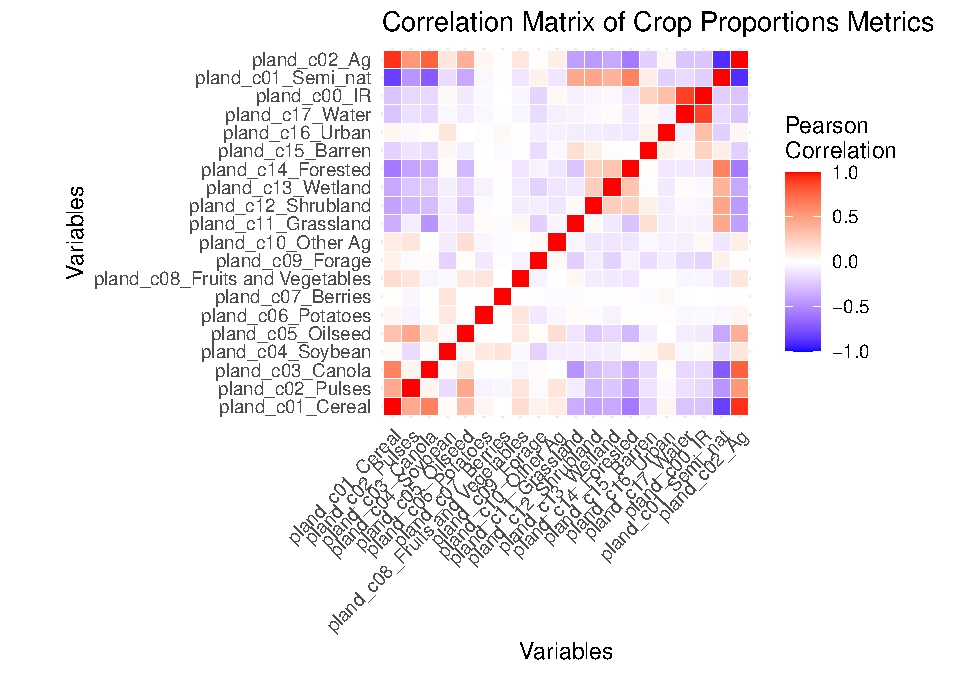
\includegraphics{NA_Analysis_files/figure-latex/unnamed-chunk-24-1.pdf}

\begin{Shaded}
\begin{Highlighting}[]
\FunctionTok{ggplot}\NormalTok{(upsa\_trd, }\FunctionTok{aes}\NormalTok{(}\AttributeTok{x =}\NormalTok{ mean\_ED, }\AttributeTok{y =}\NormalTok{ abd\_trend)) }\SpecialCharTok{+}
  \FunctionTok{geom\_point}\NormalTok{(}\AttributeTok{color =} \StringTok{"blue"}\NormalTok{, }\AttributeTok{alpha =} \FloatTok{0.3}\NormalTok{, }\AttributeTok{size =} \DecValTok{2}\NormalTok{) }\SpecialCharTok{+}  
  \FunctionTok{geom\_smooth}\NormalTok{(}\AttributeTok{method =} \StringTok{"lm"}\NormalTok{, }\AttributeTok{color =} \StringTok{"red"}\NormalTok{, }\AttributeTok{se =} \ConstantTok{TRUE}\NormalTok{, }\AttributeTok{linetype =} \StringTok{"dashed"}\NormalTok{) }\SpecialCharTok{+} 
  \FunctionTok{labs}\NormalTok{(}
    \AttributeTok{title =} \StringTok{"Relationship Between Edge Density and Trend"}\NormalTok{,}
    \AttributeTok{x =} \StringTok{"Slope of Grassland LPI (Change over Time)"}\NormalTok{,}
    \AttributeTok{y =} \StringTok{"Abundance Trend (abd\_trend)"}
\NormalTok{  ) }\SpecialCharTok{+}
  \FunctionTok{theme\_minimal}\NormalTok{() }\SpecialCharTok{+}
  \FunctionTok{theme}\NormalTok{(}
    \AttributeTok{plot.title =} \FunctionTok{element\_text}\NormalTok{(}\AttributeTok{hjust =} \FloatTok{0.5}\NormalTok{, }\AttributeTok{size =} \DecValTok{16}\NormalTok{),}
    \AttributeTok{axis.title =} \FunctionTok{element\_text}\NormalTok{(}\AttributeTok{size =} \DecValTok{14}\NormalTok{),}
    \AttributeTok{axis.text =} \FunctionTok{element\_text}\NormalTok{(}\AttributeTok{size =} \DecValTok{12}\NormalTok{)}
\NormalTok{  )}
\end{Highlighting}
\end{Shaded}

\begin{verbatim}
## `geom_smooth()` using formula = 'y ~ x'
\end{verbatim}

\includegraphics{NA_Analysis_files/figure-latex/unnamed-chunk-24-2.pdf}
\#\#\# Correlation matrix matrix of relationships / distribution of
response and explanatory variables after aggregating

\begin{Shaded}
\begin{Highlighting}[]
\NormalTok{upsa\_trd}\SpecialCharTok{$}\NormalTok{trend\_dir }\OtherTok{\textless{}{-}} \FunctionTok{ifelse}\NormalTok{(upsa\_trd}\SpecialCharTok{$}\NormalTok{abd\_trend }\SpecialCharTok{\textgreater{}}\DecValTok{0}\NormalTok{, }\StringTok{"Increase"}\NormalTok{, }\StringTok{"Decrease"}\NormalTok{)}


\NormalTok{agg\_mean\_predictors }\OtherTok{\textless{}{-}}\NormalTok{ upsa\_trd[,}\FunctionTok{c}\NormalTok{(}\StringTok{"mean\_ED"}\NormalTok{,}\StringTok{"mean\_FLPI"}\NormalTok{,}\StringTok{"mean\_GLPI"}\NormalTok{,  }\StringTok{"mean\_shdi"}\NormalTok{,  }\StringTok{"abd\_trend"}\NormalTok{, }\StringTok{"trend\_dir"}\NormalTok{)]}

\NormalTok{agg\_slope\_predictors }\OtherTok{\textless{}{-}}\NormalTok{ upsa\_trd[,}\FunctionTok{c}\NormalTok{(}\StringTok{"ED\_slope"}\NormalTok{,}\StringTok{"FLPI\_slope"}\NormalTok{, }\StringTok{"GLPI\_slope"}\NormalTok{, }\StringTok{"simp\_slope"}\NormalTok{,  }\StringTok{"shdi\_slope"}\NormalTok{, }\StringTok{"abd\_trend"}\NormalTok{, }\StringTok{"trend\_dir"}\NormalTok{)]}

\CommentTok{\#aggregated\_predictors \textless{}{-} upsa\_trd[,c("mean\_ED","ED\_slope","mean\_FLPI","FLPI\_slope","mean\_GLPI", "GLPI\_slope", "simp\_slope", "mean\_shdi", "shdi\_slope", "abd\_trend", "trend\_dir")]}

\CommentTok{\#Average }
\FunctionTok{ggpairs}\NormalTok{(agg\_mean\_predictors, ggplot2}\SpecialCharTok{::}\FunctionTok{aes}\NormalTok{(}\AttributeTok{colour =}\NormalTok{ trend\_dir), }\AttributeTok{lower =} \FunctionTok{list}\NormalTok{(}\AttributeTok{continuous =} \FunctionTok{wrap}\NormalTok{(}\StringTok{"smooth"}\NormalTok{, }\AttributeTok{colour =} \StringTok{"blue"}\NormalTok{)))}
\end{Highlighting}
\end{Shaded}

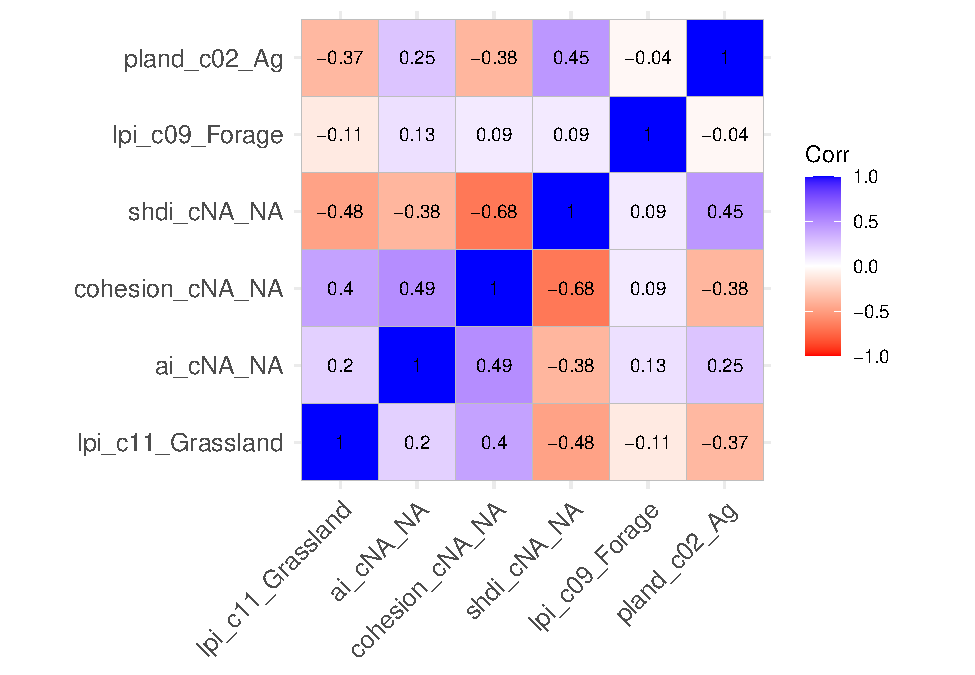
\includegraphics{NA_Analysis_files/figure-latex/unnamed-chunk-25-1.pdf}

\begin{Shaded}
\begin{Highlighting}[]
\CommentTok{\#Slope}
\FunctionTok{ggpairs}\NormalTok{(agg\_slope\_predictors, ggplot2}\SpecialCharTok{::}\FunctionTok{aes}\NormalTok{(}\AttributeTok{colour =}\NormalTok{ trend\_dir), }\AttributeTok{lower =} \FunctionTok{list}\NormalTok{(}\AttributeTok{continuous =} \FunctionTok{wrap}\NormalTok{(}\StringTok{"smooth"}\NormalTok{, }\AttributeTok{colour =} \StringTok{"blue"}\NormalTok{)))}
\end{Highlighting}
\end{Shaded}

\includegraphics{NA_Analysis_files/figure-latex/unnamed-chunk-25-2.pdf}

\begin{Shaded}
\begin{Highlighting}[]
\FunctionTok{names}\NormalTok{(upsa\_trd)}
\end{Highlighting}
\end{Shaded}

\begin{verbatim}
##  [1] "srd_id"          "mean_ED"         "ED_slope"        "ED_intercept"   
##  [5] "mean_FLPI"       "FLPI_slope"      "FLPI_intercept"  "mean_GLPI"      
##  [9] "GLPI_slope"      "GLPI_intercept"  "simp_slope"      "simp_intercept" 
## [13] "sd_shdi"         "mean_shdi"       "shdi_slope"      "shdi_intercept" 
## [17] "longitude"       "latitude"        "abd"             "abd_ppy"        
## [21] "abd_ppy_lower"   "abd_ppy_upper"   "abd_ppy_nonzero" "abd_trend"      
## [25] "abd_trend_lower" "abd_trend_upper" "trend_dir"
\end{verbatim}

\section{Model Runs}\label{model-runs}

Current work in progress\ldots{}

I have the data frame and predictors set up to be able to run models.

I need to determine which predictors I will use in candidate models
(mean vs slope). Also, I need to determine a strategy for how I will
model.(How can I include abundance, spatial dependencies?, error
structure?)

\end{document}
